%**************************************************%
% Author     : Fatih Selim Yakar                   %
% ID         : 161044054                           %
% Title      : Systems Programming Final Report    %
% Instructor : Erchan Aptoula                      %
%**************************************************%

\documentclass{article}

\usepackage[utf8]{inputenc}
\usepackage[margin=1in]{geometry}
\usepackage[titletoc,title]{appendix}

\usepackage{graphicx}
\graphicspath{ {.} }

\usepackage{minted}
\usemintedstyle{borland}

\usepackage{biblatex}
\addbibresource{references.bib}

% Title content
\title{\textbf{CSE344 System Programming Final Project Report}}
\begin{document}

\maketitle

% Center
\begin{center}
    \textbf{Student:}Fatih Selim YAKAR \\
    \textbf{Student No:}161044054 \\
    \textbf{Instructor:}Erchan APTOULA
\end{center}

\newpage

%Overview
\section{Overview}
\par{In this assignment, I did synchronization and exchange between an indefinite number of client and server(and their threads) through sockets and pthread tools. The context was as follows: There was a file with the server's input. And this file contained a graph. The desired graph was to be read by the server and turned into a data structure, and then the path from the client, between 2 nodes, was to response the requests. There would be another system inside the server. This system is as follows: The server that will occur in the server main thread and calculater threads will transmit each incoming connection to the threads, then if there is a path in the cache structure, it will read it with the writers-readers paradigm, calculate it if not, then write it to the cache and send it to the client. On the other hand, I used an additional thread to make the server system dynamic. This additional thread had its own special condition variable and mutex. I created global arrays, so that all threads were able to reach. I created mutex for the number of threads for critical sections. For some cases, I solved the wait by creating a condition variable as many as the number of threads. For finishing in the Ctrl-c state and the nominal state, I used condition variables first. In any case, I freed all the resources while the program was over. You can find the details below.}

% Synchronization Problem Between Threads
\section{Synchronization Problem Between Threads}
\par{In case of this homework, there are main thread also there are calculater threads. Threads have to work in parallel among themselves. On the other hand, in the critical section, it is necessary to add a connection fds to the queues of each thread with the main thread and to get a fd from the queues by the calculater threads.}

% Providing critical section
\subsection{Providing critical section}
\par{I used mutex to provide the critical section. If I tried to do this for all threads with a single mutex, not all threads would work at the same time. I created a separate mutex for each thread to ensure that all threads can work in parallel, and while adding a queue socket fd to the main thread, I locked the necessary thread's mutex and performed the necessary operation and unlocked it after doing the operation. Likewise, within calculater thread, each calculater thread made the process of path calculating with writers and readers paradigm with accessing cache.}


\subsection{Waiting with condition variables for queues}
\par{I created a fd queue for each calculater thread. When these queues are full, the main thread should not add socket fd to the queue and the florist should not receive socket fd from the queue when the queue is empty. So in these cases, it should wait for it to fill up or empty. I did not use condition variable to be full since I dynamically built queues. But since the calculater threads should wait if the queue is empty, I have defined the condition variable as many as the number of threads. I did pthread cond signal when adding socket fd to main thread queue. And in the calculater thread I made pthread cond wait if the size of the queue was zero so I solved the sync issue in the queues.}


\subsection{Readers-Writers paradigm for accessing cache}
\par{In reaching the cache, I used the writers readers paradigm to get writer priority or reader priority or not to give any priority (Bonus part). In order to implement the Writers-Readers paradigm, I used int variables named 4 active\_readers, active\_writers, waiting\_readers and waiting\_writers. In addition, I used 2 ok\_to\_read and ok\_to\_write condition varible and finally 1 mutex named rw\_mutex.I implemented the paradigm as in the figure I showed below. (For the -r parameter, I edited it by doing a few if it was processed in the lesson.)}

\newpage 

\begin{center}
    \textbf{Writers-Readers Figure \\}
    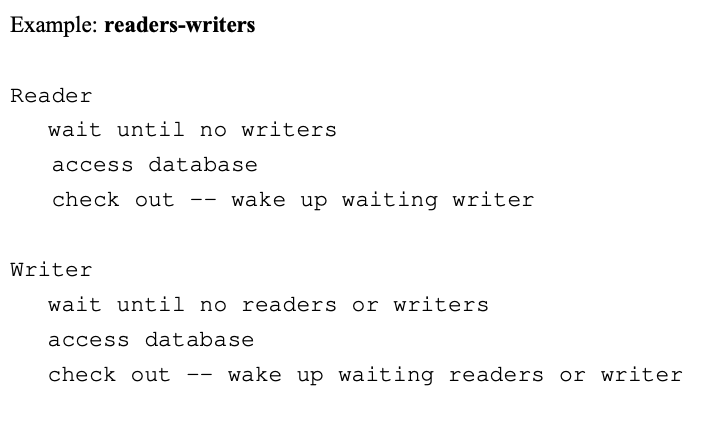
\includegraphics[scale=0.6]{writers-readers.png} \\[0.5in]
\end{center}



\section{In Case Of SIGINT(ctrl-c)}
\par{Termination of the program (that is, SIGINT signal coming) was designed as follows: I have defined a sigint handler function with sigaction for the server program to exit. When I entered this function, I just printed an information that it was caught and then changed the global sigint\_flag from 0 to 1. Then, since the main thread condition was while (sigint\_flag == 0), I stopped receiving the main thread immediately. After that, I sent a cond signal to all threads to wake up the threads sleeping under the main thread. The threads receiving the signal entered and exit the finishing condition following the cond wait condition. After the expected threads with the pthread\_join function in Main, I made a refund of the resources.}

\section{Cache Data Structure}
\par{For the cache data structure, I created a data structure similar to Hash table using the combination of 2 data structures. I have defined a CacheNode array with as many elements as Vertex in the structure. Then, every array element became a structure containing the next pointer, end node and path, like the linked list node. Thus, in the case of $0->20$ searches, it went to the CacheNode at index 0 and looked at the equation of its endnode, and went through the linked list by making item $=$item$->$next, thus accessing and writing $O (n)$ [n = path number in that index].}

\section{Graph Data Structure}
\par{For the Graph data structure, I used a mix of adjacency list and adjacency matrix, structurally the same as the adjacency list, but in the rest of the arrays, I used a dynamic array, not a linked list. So I used a 2d matrix like an adjacency list.}

\newpage

\section{Dynamic thread pool}
\par{I used 1 thread 1 mutex and 1 condition variable to increase the dynamic thread pool, that is, to increase the capacity of the system's threads by 75\% and above 25\% capacity. As soon as the pool I used was working in thread and main, I made mutex lock and unlock to provide critical region as normal. I sent pthread\_cond\_signal so that the main thread can work with the pool thread in every loop. I did pthread\_cond\_wait on the pool thread with the condition of While (busy state is less than 75\% or thread count has reached the limit). Then I created new threads with pthread\_create, increasing 25\% if it exits this pthread\_cond\_wait loop.}


\section{Functions Used And Their Explanations}
\subsection{server.c}
\begin{itemize}
    \item \textbf{static void create\_daemon()}:Transforms the current process to daemon.
    \item \textbf{void get\_request(int sockfd,int thread\_index)}:Function that takes the path request from the client and calculates the path according to the request. Applies the Writers-readers thread structure.
    \item \textbf{void open\_socket(int port)}:Opens a new socket.
    \item \textbf{void *calculator\_threads (void *arg)}:Thread function that processes connections (accepted fds) from the main thread and returns to the client.
    \item \textbf{void *pool\_thread(void *arg)}:Thread function that increases the number of threads by 25\% if it looks at the thread size and operates at over 75\%. 
    \item \textbf{void sigint\_handler(int signum)}:SIGINT handler function.
    \item \textbf{int main(int argc,char *argv[])}:The files are opened, the daemon process is created, then the sockets are opened and after all threads are started, main thread runs until the sigint signal comes.
    
\end{itemize}

\subsection{client.c}
\begin{itemize}
    \item \textbf{void send\_request(int sockfd,int source,int destination)}:Sends request to get path.
    \item \textbf{int main(int argc,char *argv[])}:Opens sockets and sends path request according to command line arguments.
\end{itemize}

\subsection{cache.c/h}
\begin{itemize}
    \item \textbf{struct Cache* create\_cache(int capacity)}:Creates the cache stucture and returns.
    \item \textbf{int find\_end\_node\_in\_path(char *path)}:Finds the end node of char* path by seperating tokens.
    \item \textbf{int find\_first\_node\_in\_path(char *path)}:Finds the first node of char* path by seperating tokens.
    \item \textbf{void add\_path\_in\_cache(char* path,struct Cache* cache,int output\_fd)}:Add new path in the linkedlist array.
    \item \textbf{char* find\_path\_in\_cache(int start\_node,int end\_node,struct Cache* cache)}:Finds the path in the cache.
    \item \textbf{void free\_cache(struct Cache* cache)}:Frees the cache data structure.
\end{itemize}

\newpage

\subsection{graph.c/h}
\begin{itemize}
    \item \textbf{int find\_maximum\_index(char* file\_name,int output\_fd)}:Finds and returns the maximum indexed node to determine the number of nodes.
    \item \textbf{struct Graph* initialize\_graph(char* file\_name,int output\_fd)}:Initializes the graph reading line by line.
    \item \textbf{int add\_node(int first\_node,int second\_node,struct Graph* graph)}:Adds node in graph.
    \item \textbf{int is\_there\_node(int first\_node,int second\_node,struct Graph* graph)}:Control is there node in graph.
    \item \textbf{int BFS(struct Graph* graph, int s, int d, int* parent\_array)}:BFS that stores the parents.
    \item \textbf{int find\_path\_in\_graph(struct Graph* graph, int s, int d,char *return\_path)}:Cover function of BFS.
    \item \textbf{void free\_graph(struct Graph* graph)}:Frees the graph structure.
    
\end{itemize}

\subsection{input\_output.c/h}
\begin{itemize}
    \item \textbf{unsigned long get\_time\_microseconds()}:gets time according to microseconds.
    \item \textbf{void print\_error(char error\_message[])}:Prints error in the STDERR.
    \item \textbf{void print\_string\_output\_fd(char string[],int output\_fd)}:Prints string in the output\_fd.
    \item \textbf{void print\_string(char string[])}:Prints string in the output\_fd 
    
\end{itemize}


\subsection{queue.c/h}
\begin{itemize}
    \item \textbf{struct Queue* create\_queue(int capacity) }:Creates the queue and returns it.
    \item \textbf{int is\_empty(struct Queue* queue)}:Controls is empty.
    \item \textbf{int is\_full(struct Queue* queue)}:Controls is full.
    \item \textbf{int add\_item(struct Queue* queue,int item)}:Adds item to rear.
    \item \textbf{int get\_item(struct Queue* queue)}:Gets item in the front.
    \item \textbf{int get\_item\_and\_delete(struct Queue* queue)}:Gets item in the front and deletes it (pop).
    \item \textbf{void free\_queue(struct Queue* queue)}:Frees the queue structure.
    
\end{itemize}

\newpage

\section{Sample Running Screenshots \\}
\begin{center}
    \textbf{Makefile with -Wall -Wextra -pedantic \\}
    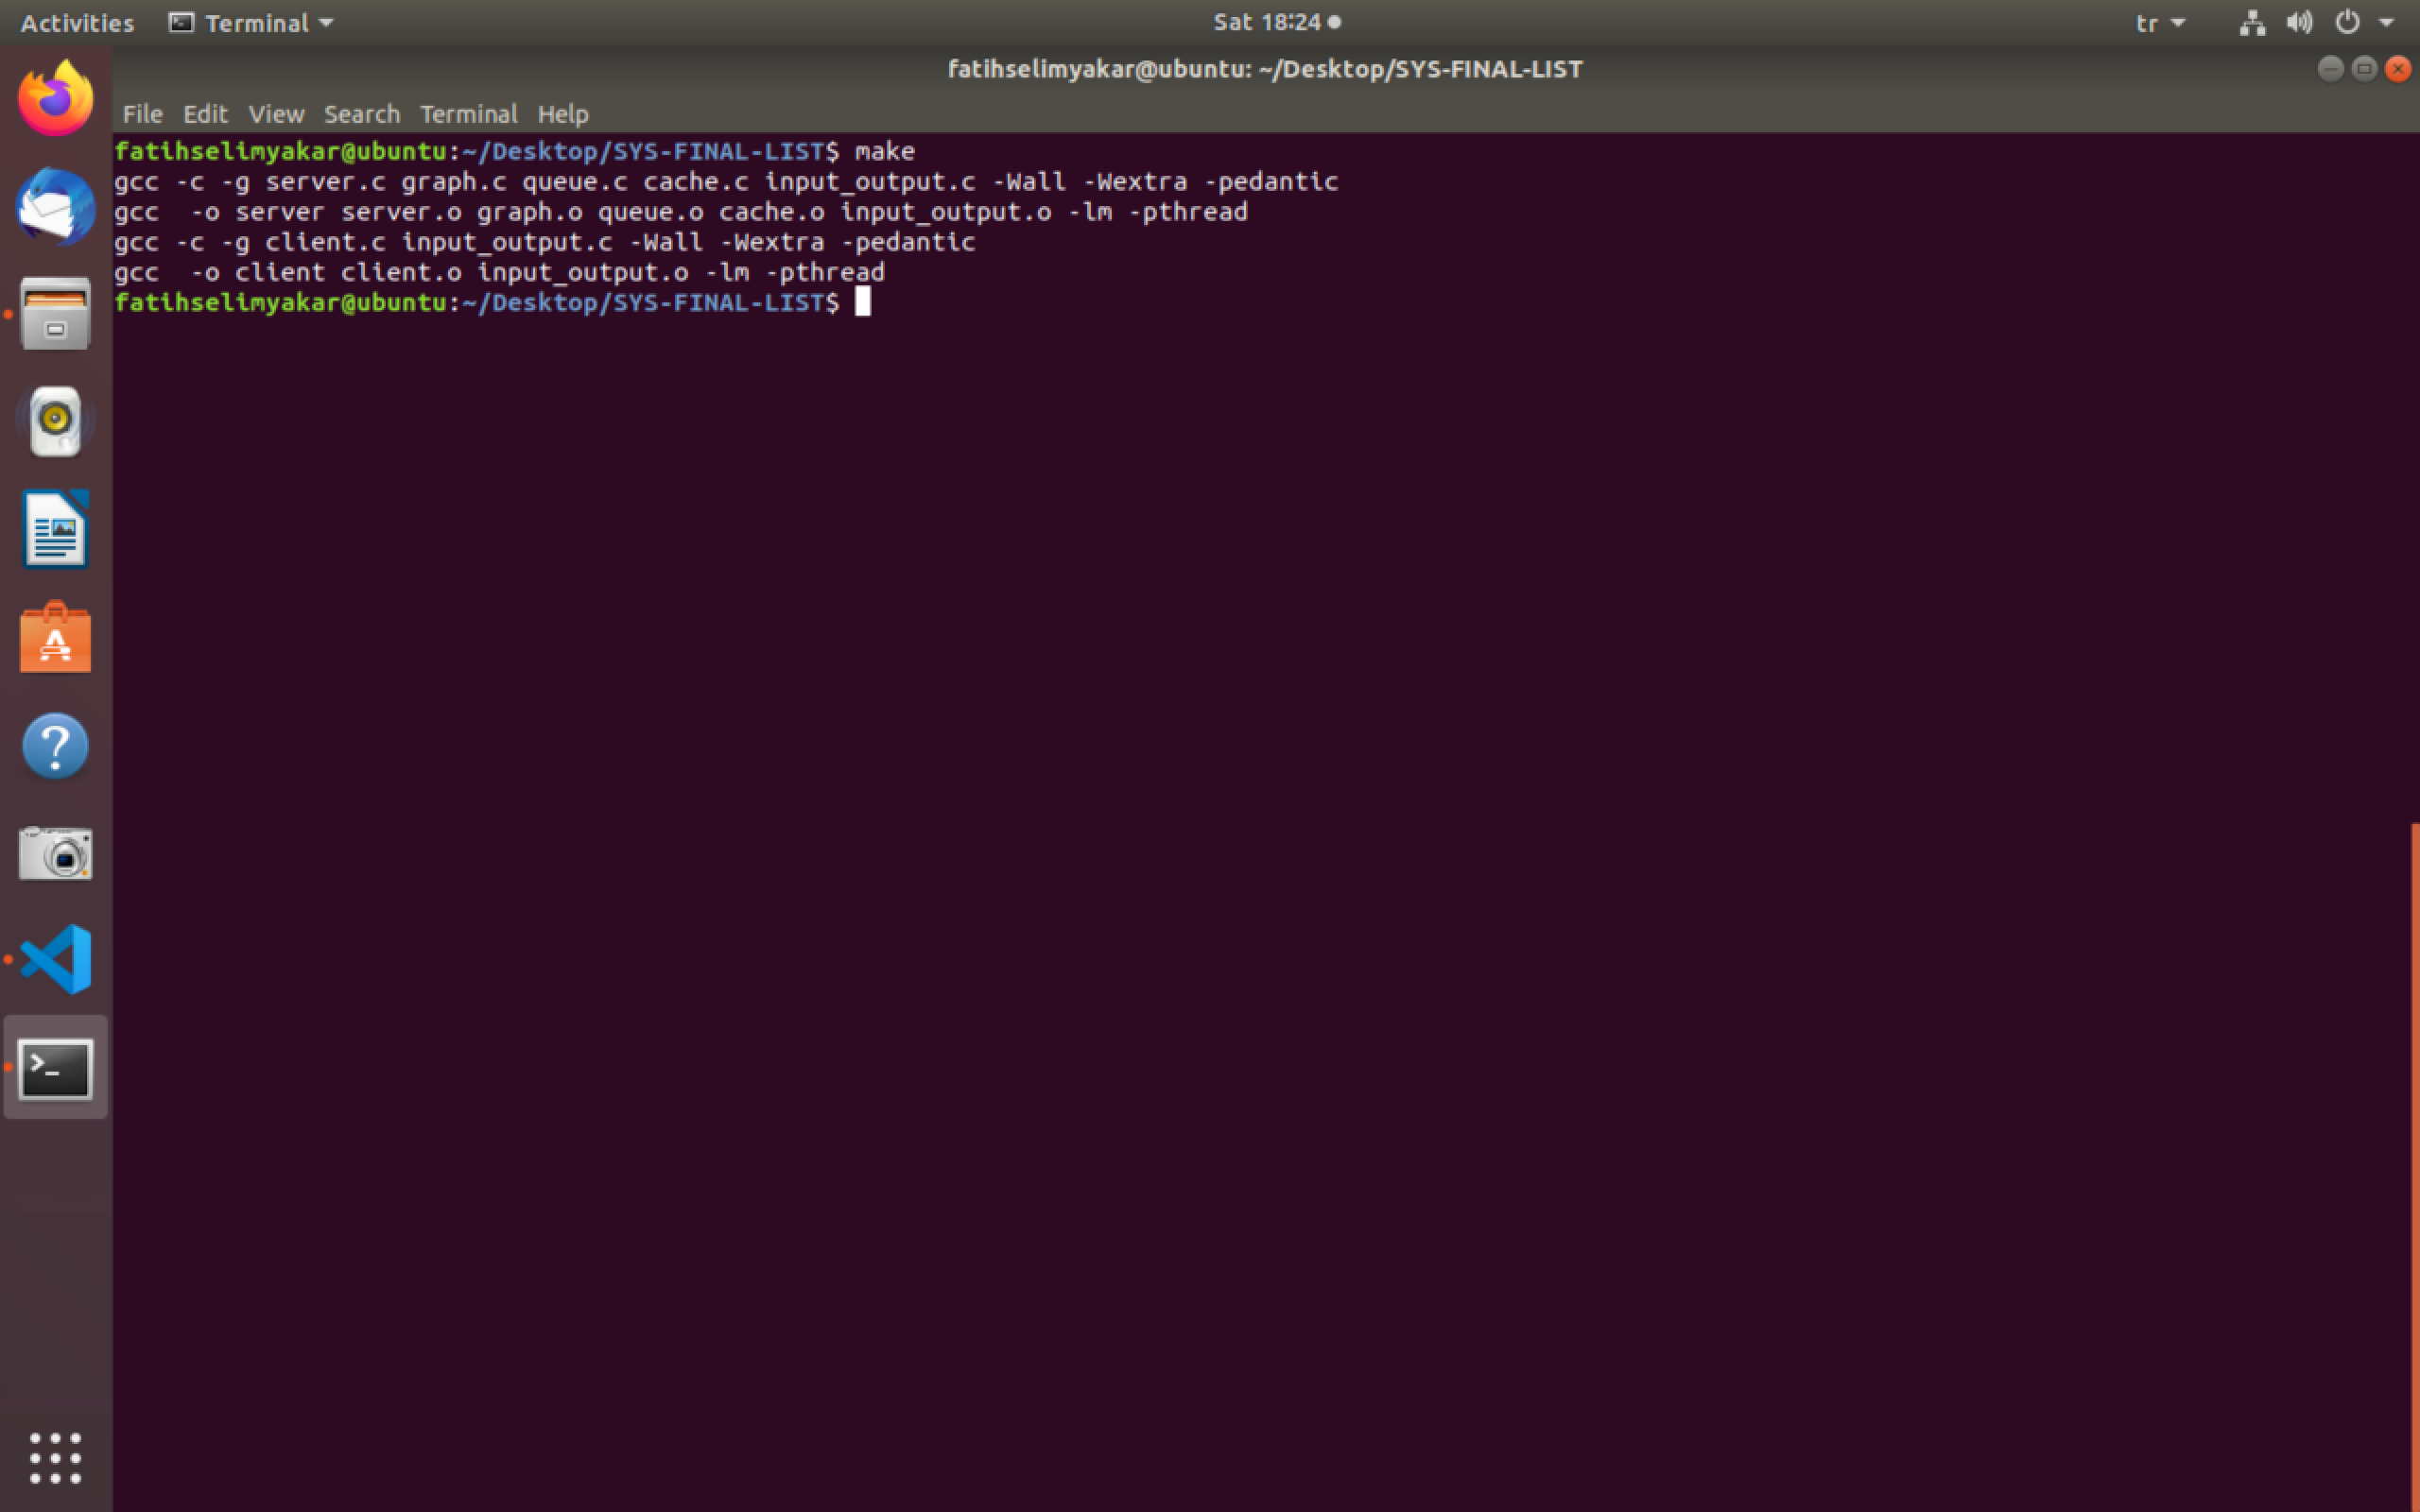
\includegraphics[scale=0.32]{makefile.png} \\[0.5in]
    \textbf{Running and finishing server with valgrind} \\
    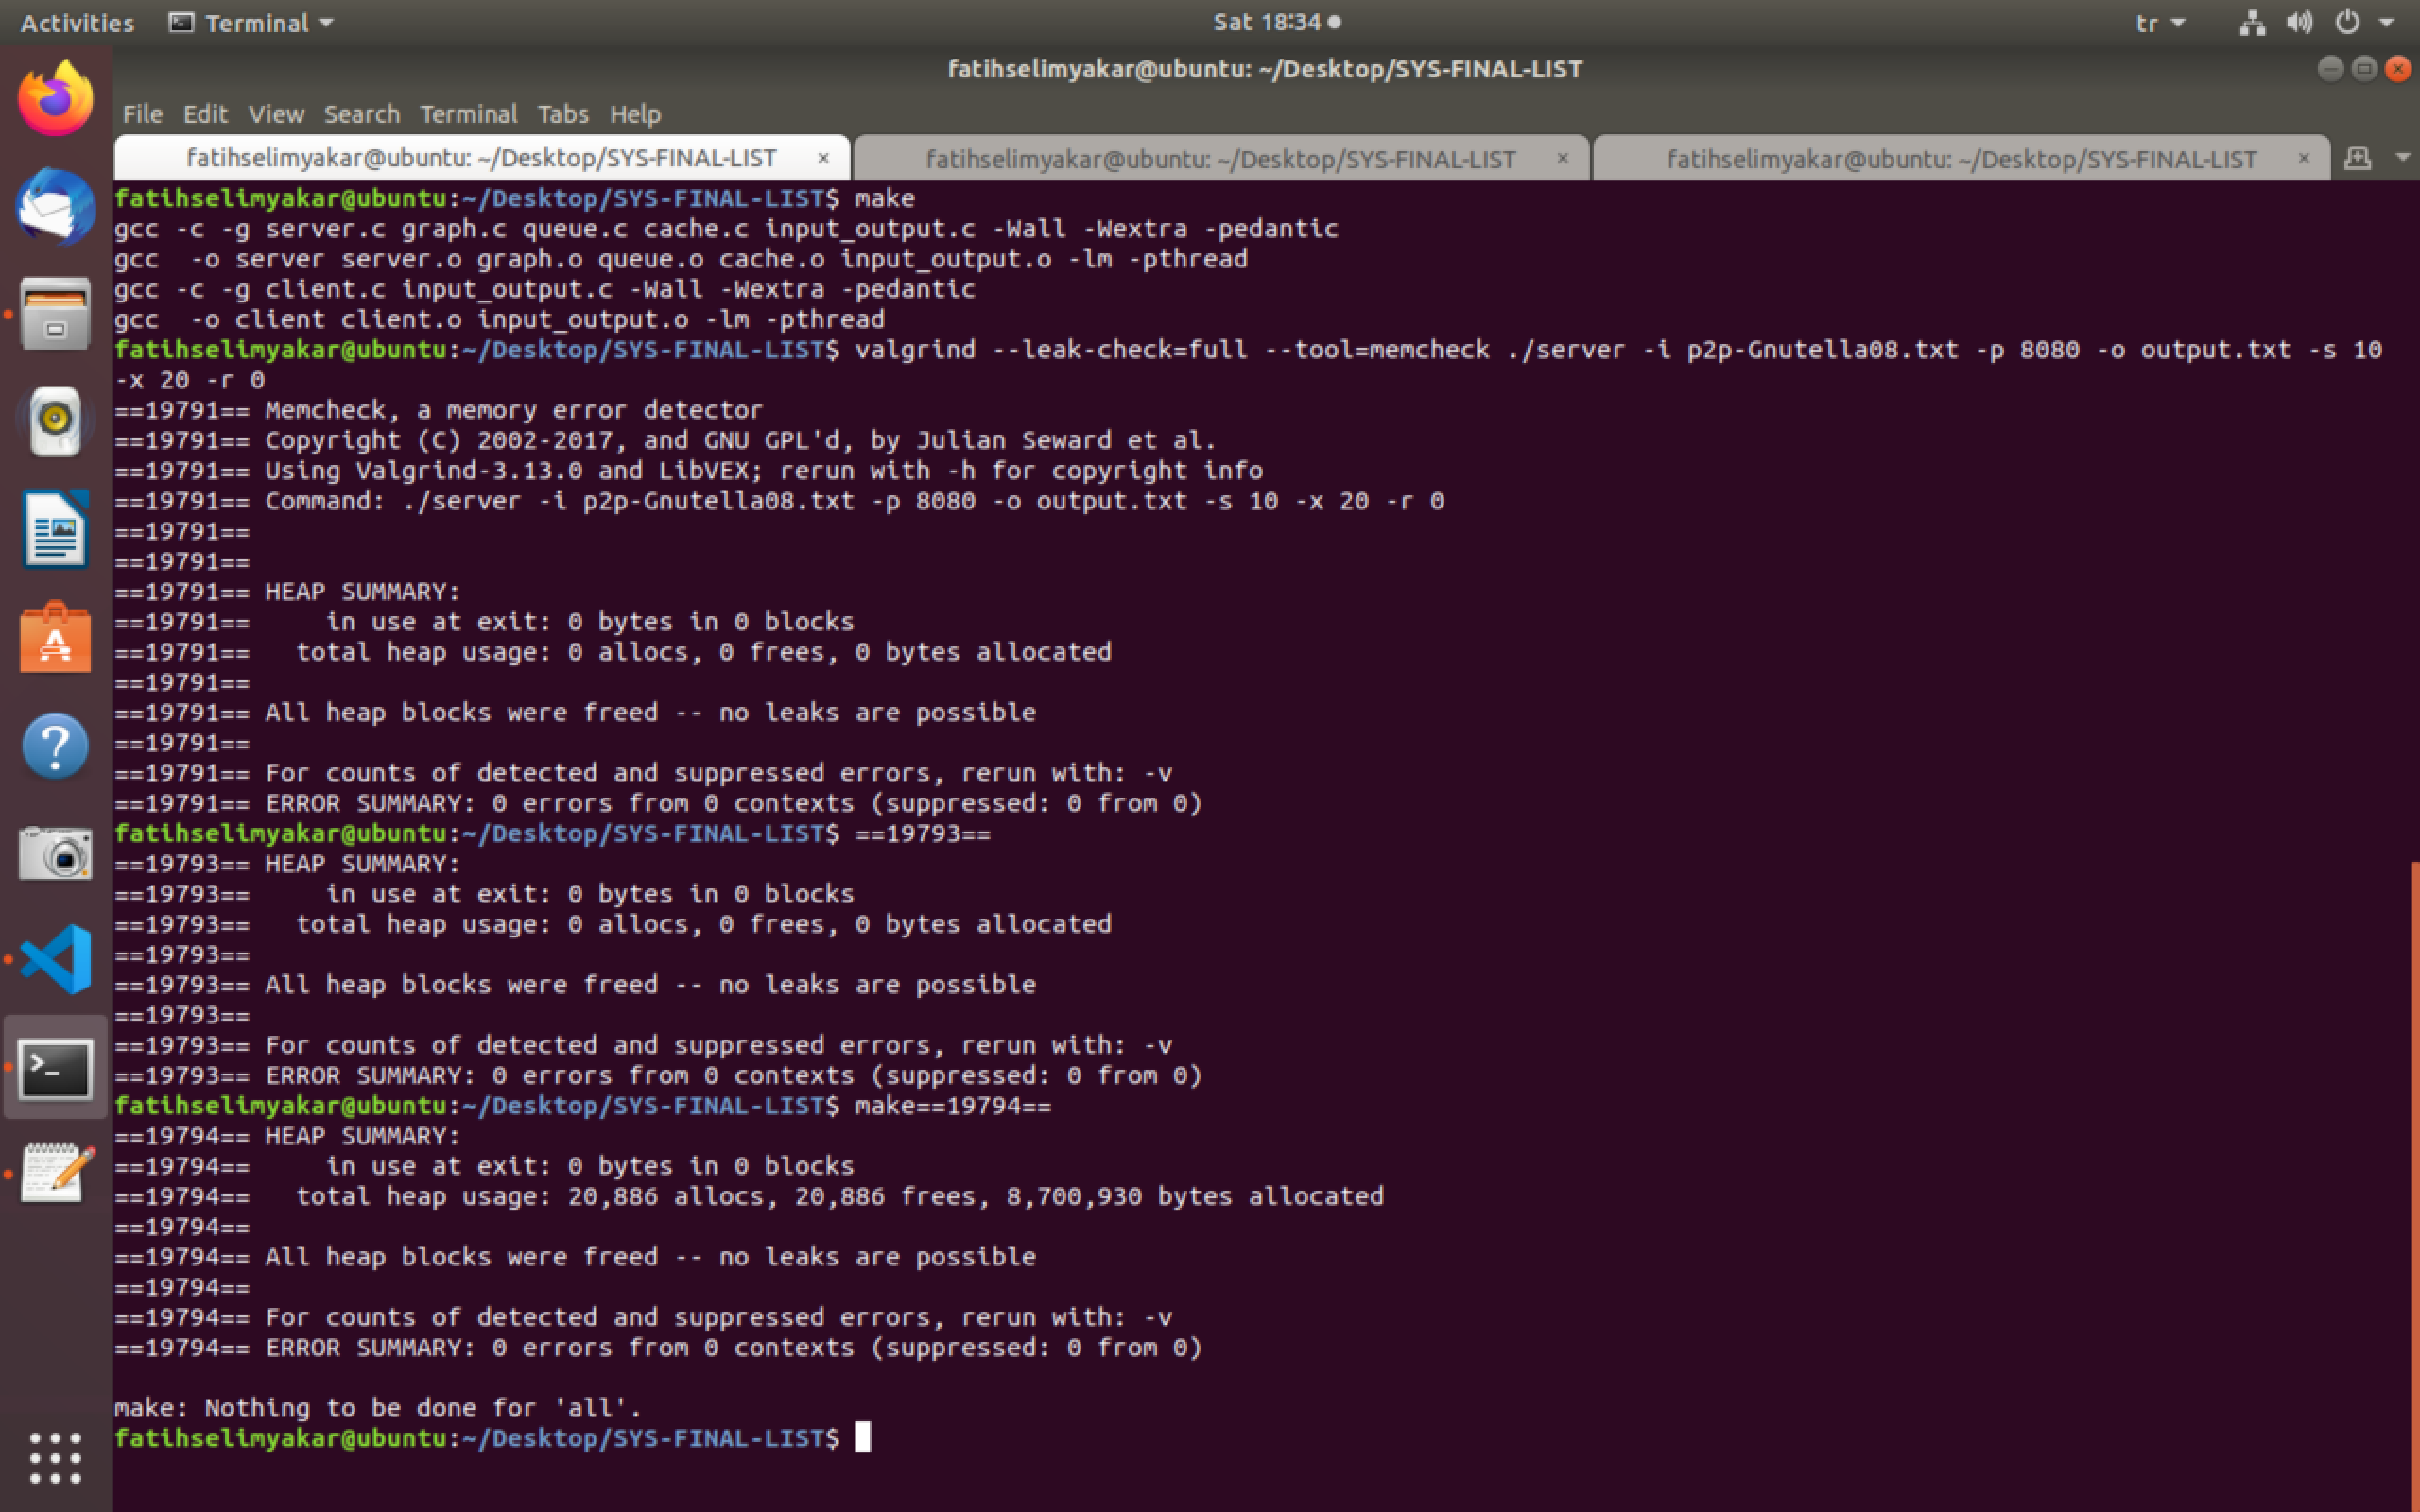
\includegraphics[scale=0.32]{server.png}
    \newpage
    \textbf{Running client with valgrind} \\
    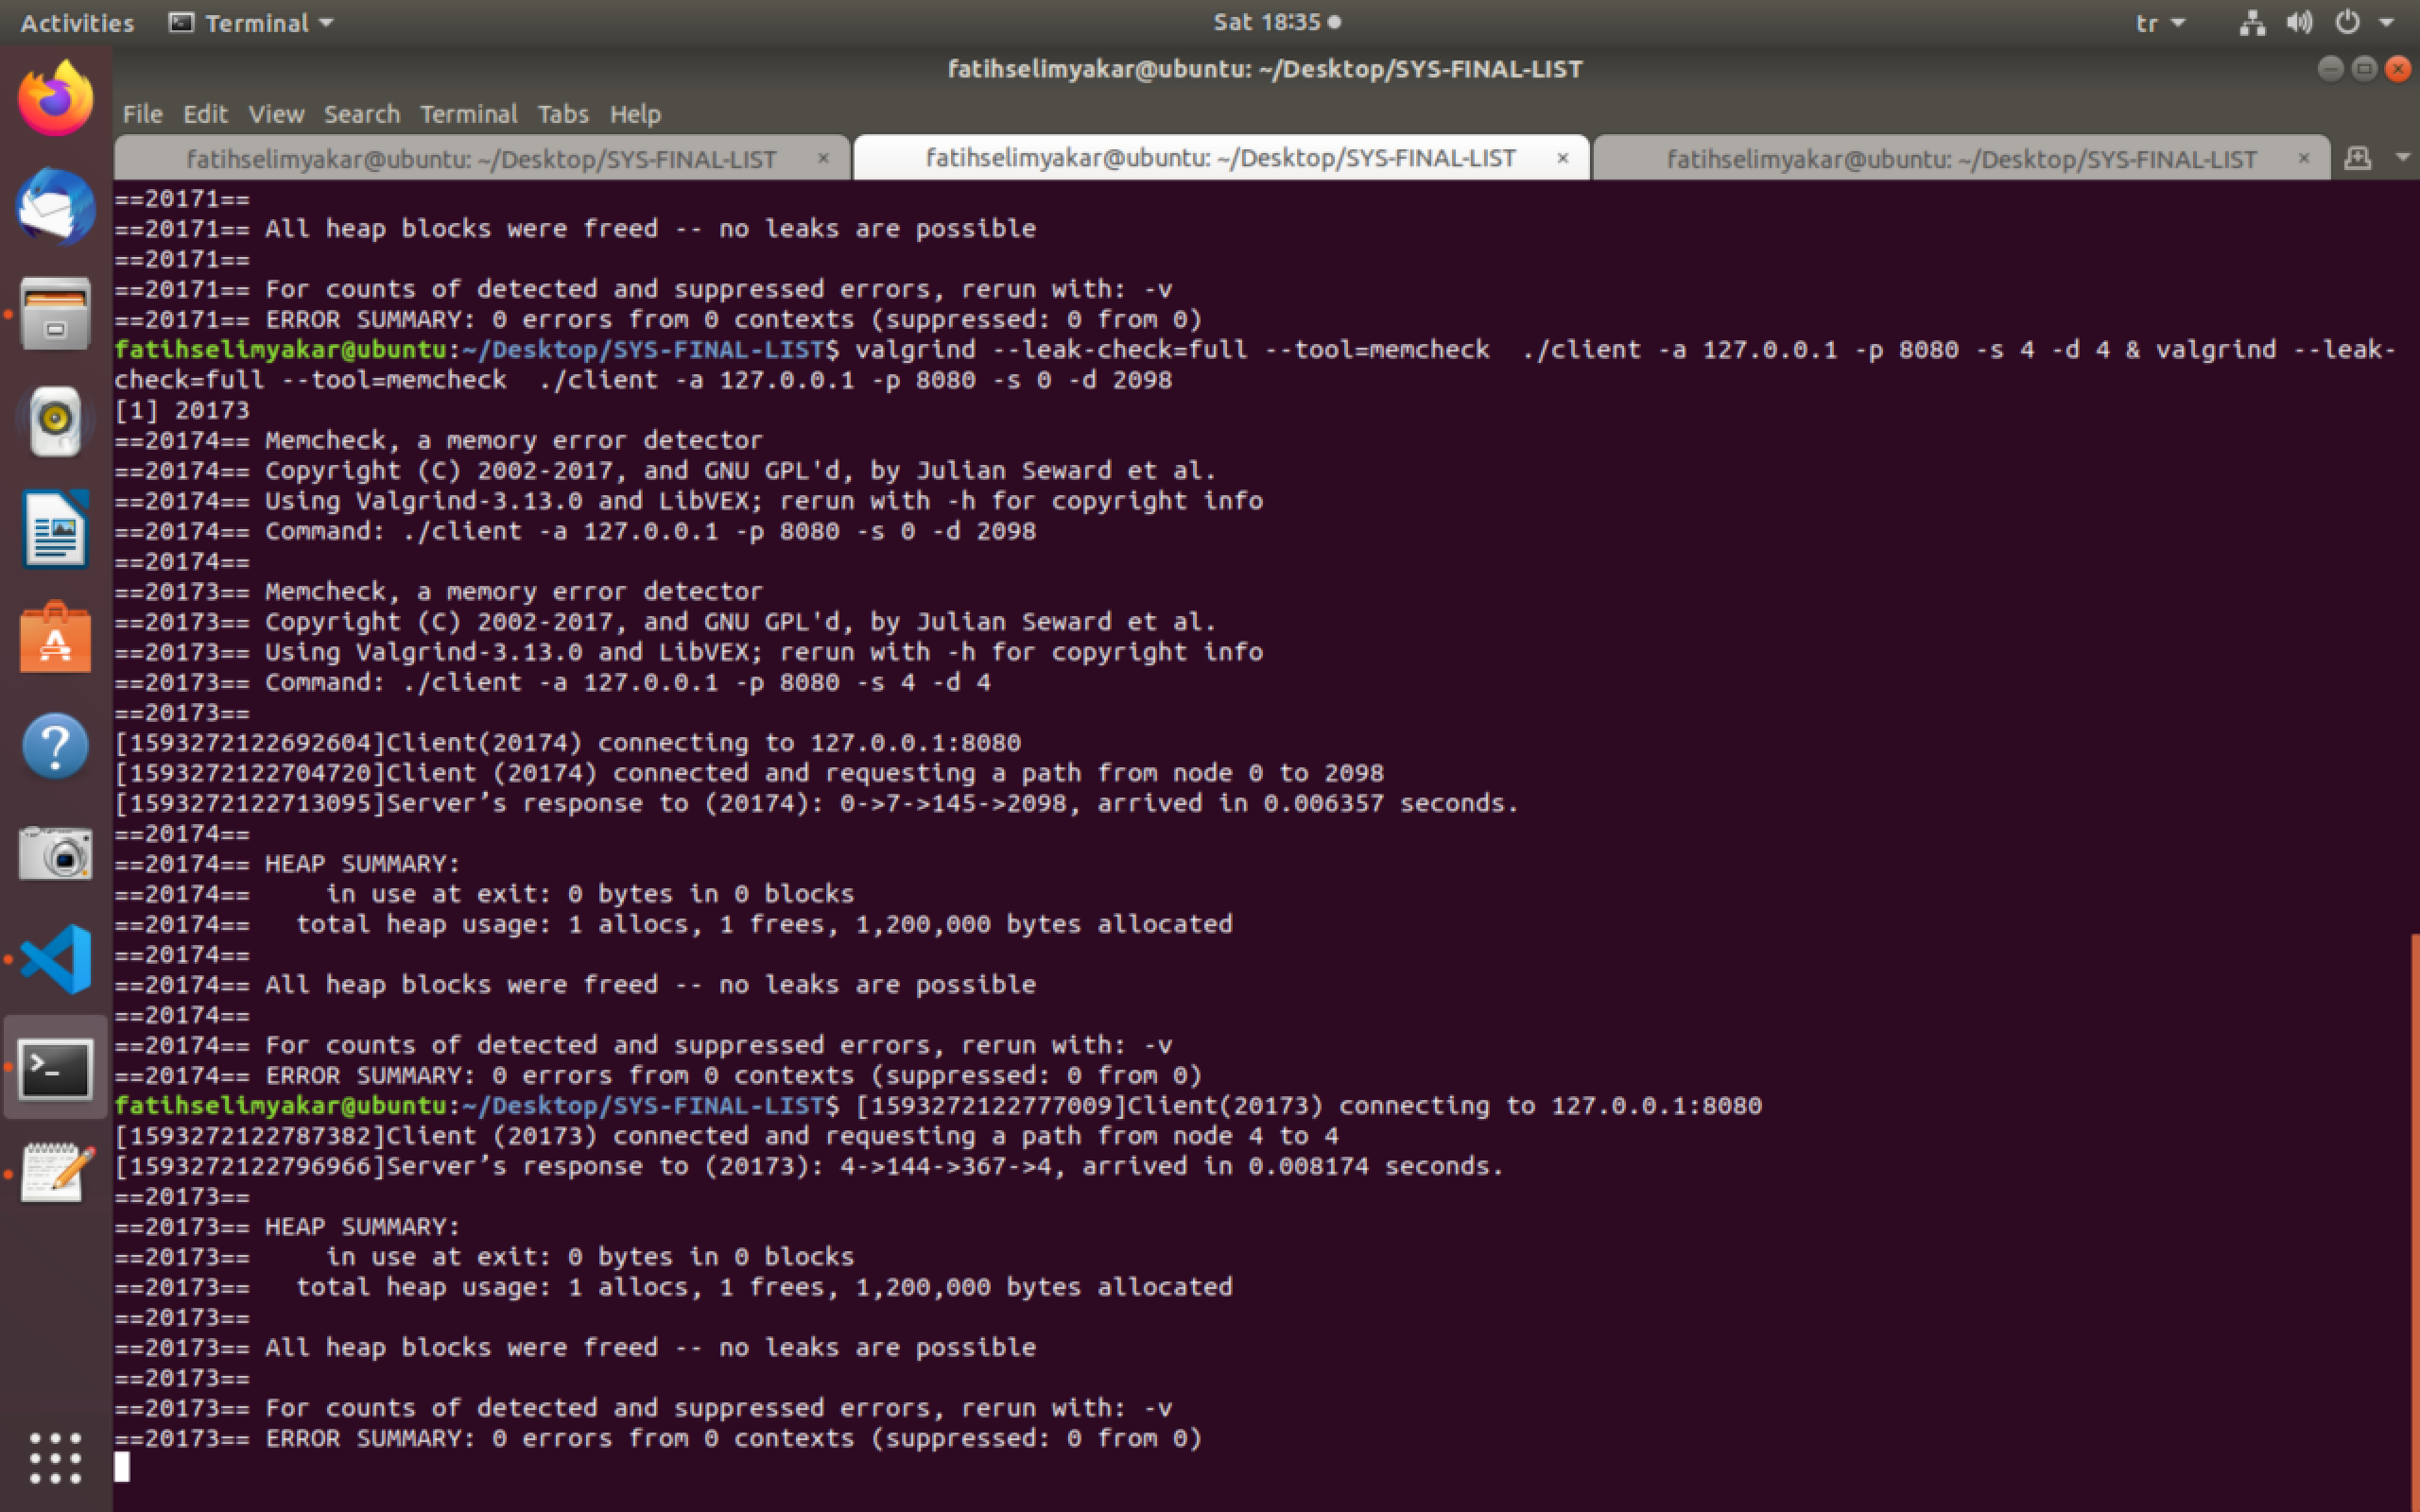
\includegraphics[scale=0.32]{client.png} \\[0.5in]
    \textbf{Output log file after the ctrl-c} \\
    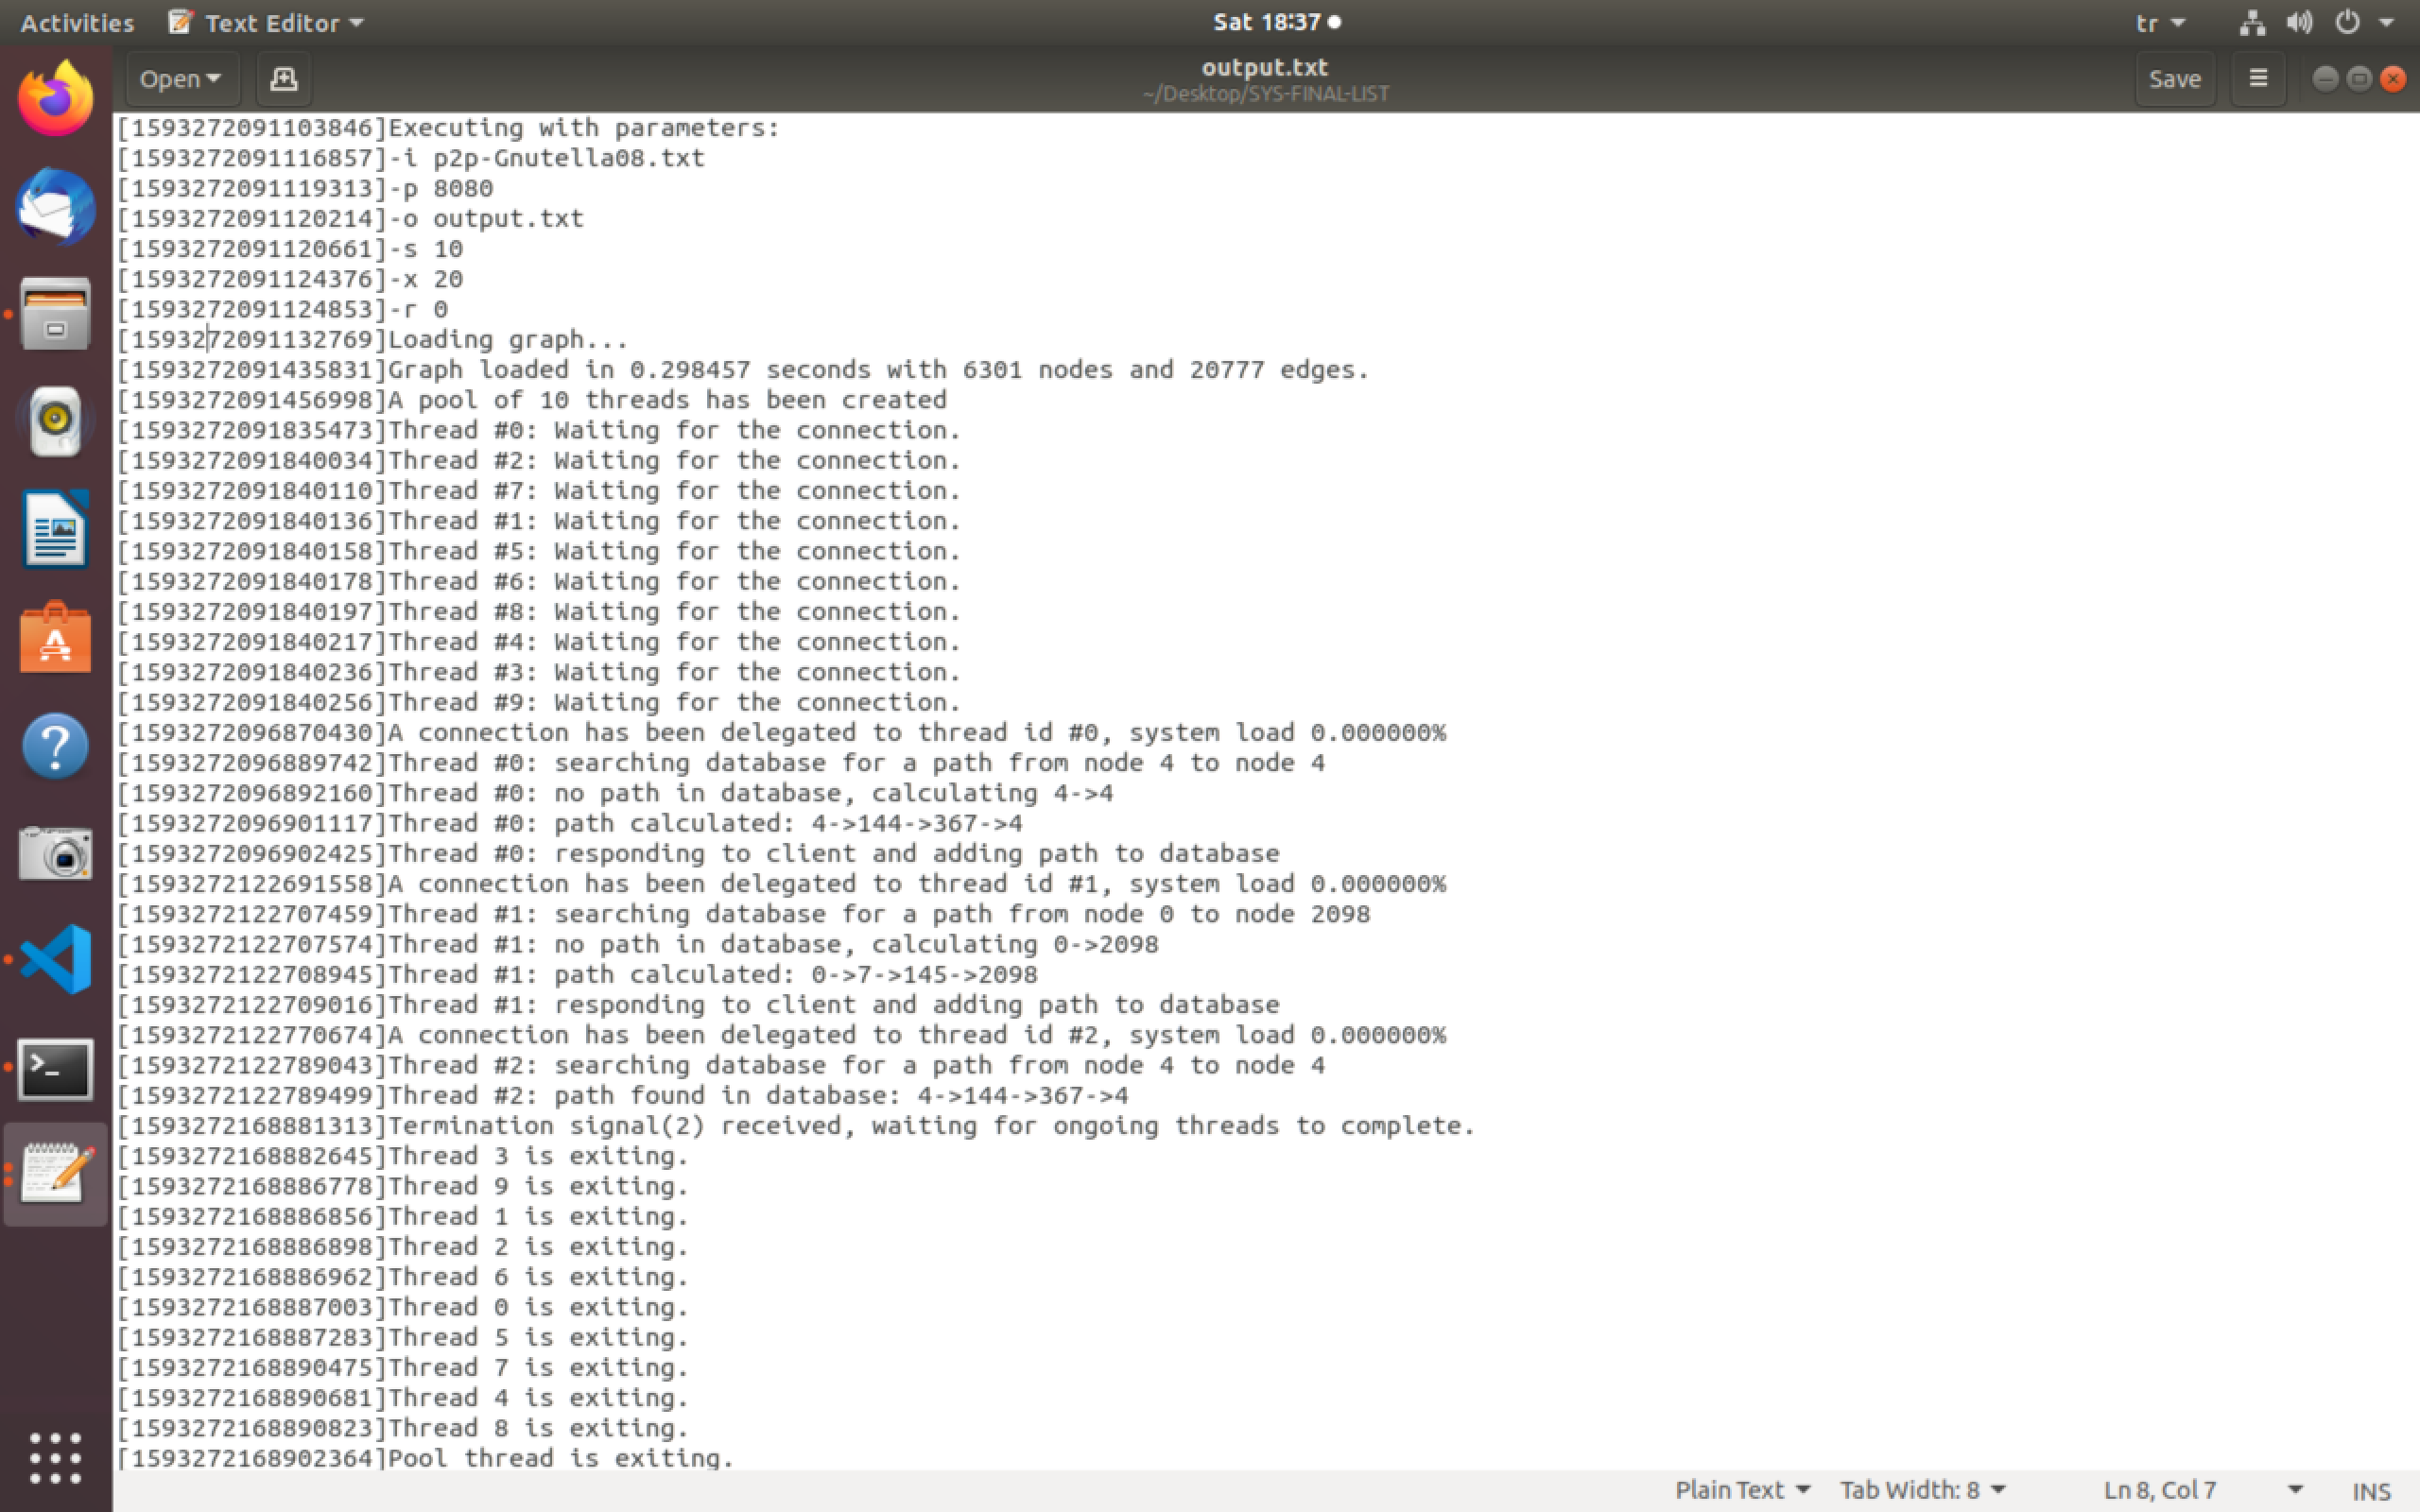
\includegraphics[scale=0.32]{output.png}
\end{center}

\newpage

\section{Notes}
\begin{itemize}
    \item The program started with 2 and 3 threads due to the extension rule up to 25\% will not extend due to 2/4 and 3/4 being less than 1.
    \item There are limits to 999999 characters for the path when writing and reading socket.
    \item It creates an empty file with the name "running" to prevent a 2nd program from running. It prevents restarting because it cannot be deleted in an unexpected error (seg. Fault etc.). It is necessary to delete "running" to try again
    \item It has been tried as 5-25 threads with wiki-Talk.txt and soc-LiveJournal1.txt graphs on the given website.
    \item Nodes are accepted from 0 to node number-1. So node must have 0,1,2,3,4 nodes for size = 5.
    \item Due to the permissions on the computer, it may be necessary to run with sudo.
    \item After the sigint signal is thrown with "kill -2 pid", it should be waited for a while to run again. In this case, although the sockets are closed sometimes, the socket may generate creation error.
    \item A bonus part of 30 points has been implemented.
\end{itemize}
    

\end{document}
